\documentclass[11pt]{article}

\usepackage[utf8]{inputenc}
\usepackage[margin=0.8in]{geometry}
\usepackage{graphicx}
\graphicspath{{data/}}
\usepackage{float}
\usepackage{amsmath}
\usepackage{amssymb}
\usepackage{setspace}
\usepackage{enumitem}
\usepackage{titlesec}
\usepackage{siunitx}
\usepackage{comment}
\usepackage{caption}
\usepackage[version=4]{mhchem}
\usepackage{minibox}
\usepackage{gensymb}

\newenvironment{tight_enumerate}{
    \begin{enumerate}[label=(\alph*)]
    \setlength{\itemsep}{3pt}
    \setlength{\parskip}{0pt}}
    {\end{enumerate}}
\DeclareSIUnit{\msun}{
    \text{$M_{\odot}$}
}

\titleformat*{\section}{\large\bfseries}
\titleformat*{\subsection}{\normalsize\bfseries}

\title{\vspace{-2.5em} \textbf{Homework 5}}
\author{Justin Kang \\ AST 381: Star Formation}
\date{\vspace{-0.75em} November 20, 2018}

\begin{document}
\maketitle
\singlespacing
\pagenumbering{gobble}
\sloppy


\vspace{-2.5em}
\section*{Problem 1. The $\alpha$ and the $\Omega$.}
Consider a disk having a dimensionless viscosity $\alpha$. The disk accretes at a steady rate $\dot{M}$, where $\dot{M} = -3\pi\Sigma\nu$ and for an "alpha" disk with scale height $h$, $\nu = c_{s}h\alpha$. The disk cools radiatively. Neglect the difference between the effective temperature of the disk $T_\text{eff}$ (which is nothing more than a convenient way of stating what the emitted flux is) and the actual gas kinetic temperature $T$. Take the gas to have sound speed $c_s$ and angular frequency $\Omega$, both of which vary with disk radius $r$.

You will need to make use of the relation between the power emitted per unit area and the accretion rate:
\[\sigma_{sb}T_\text{eff}^{4} = \frac{3}{8\pi}\frac{GM_{*}\dot{M}}{r^{3}}.\]

\begin{tight_enumerate}
\item Find how $h/r$ scales with $r$, where $h$ is the disk vertical scale height. Sketch how the disk looks.

\item Find how the surface density $\Sigma$ scales with $r$. 

\item Find how the disk mid-plane density $\rho$ scales with $r$. 

\item Find an approximate expression for how long it takes a pressure disturbance to equilibrate away. Call this time $t_z$, and express it as simply as possible.

\item Find an approximate expression for how long it takes a temperature disturbance to equilibrate away. Call this time $t_{cool}$ and express it in terms of $\alpha$ and $\Omega$.

\item Find an approximate expression for how long it takes a mass disturbance (say, a local bunching of material) to viscously diffuse away. Call this time $t_{visc}$, and express it in terms of $\alpha$, $\Omega$, and $h/r$. Arrange $t_z$, $t_{cool}$, and $t_{visc}$ in increasing order.

\item Find an expression for the critical radius $r_{crit}$ beyond which Toomre's $Q < 1$. Express the result in terms of $\alpha$, $M$, and $\dot{M}$. Alpha disks are generically unstable at large radii, leading some to surmise that the outer peripheries of quasar accretion disks/protostellar accretion disks are fertile breeding grounds for starbursts/binary companion stars or brown dwarfs.
\end{tight_enumerate}

\subsection*{Solution 1}
\begin{tight_enumerate}
\item We follow the same derivation as in class. Assume that the disk is axisymmetric ($\frac{\partial}{\partial\phi} = 0$), in steady state ($\frac{\partial{u}}{\partial{t}} = 0$), $M_{disk} \ll M_{*}$, and isothermal ($P = \rho{c_s^2}$). The $z$-component of the momentum equation gives us 
\[\frac{1}{\rho}\frac{dP}{dz} = \frac{GM}{r^{2}}\sin\theta.\]
Let $\int_{-\infty}^{\infty}dz \equiv 2h$ and $\int_{-\infty}^{\infty}{\rho}dz = 2h\rho \equiv \Sigma$. Using these and our assumptions, the momentum equation reduces to 
\[\frac{P}{{\rho}c_s^2} = \frac{GM}{r^2}\frac{h}{r} \implies \frac{c_s^2}{h} = \frac{GM}{r^2}\frac{h}{r} \implies c_s^2 = \frac{GM}{r}\frac{h^2}{r^2}.\]
Rearranging and taking the square root, we arrive at our desired equation.\\
\minibox[frame]{$\therefore$ $\frac{h}{r} = c_{s}\sqrt{\frac{r}{GM}}$.}

\begin{figure}[H]
\centering
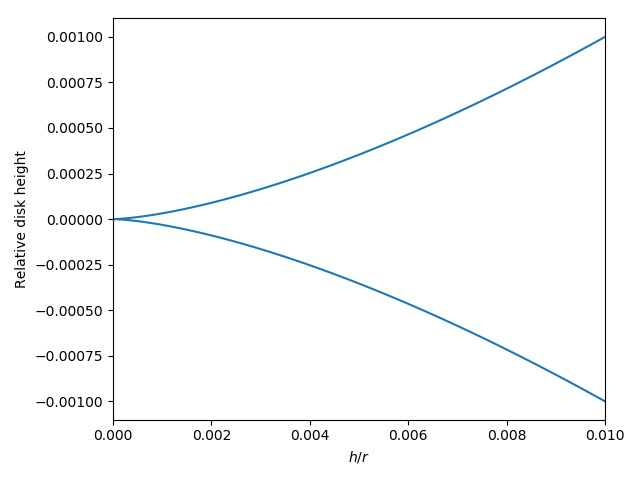
\includegraphics[height=0.275\textheight]{disk.png}
\vspace{-1em}
\caption{The general shape of the disk. Here $h/r$ is set with $h$ as a constant and varying $r$. The $y$-axis captures only the general shape of the disk, with no regard for constants.}
\end{figure}

\item We know that $\dot{M} = -3\pi\Sigma\nu$, and $\nu = \alpha{c_s}h$. From (a), we know that $h = c_{s}\Omega = c_{s}\sqrt{\frac{r^3}{GM}}$. Substituting in $\nu$ to $\dot{M}$, we find that 
\[\dot{M} = -3\pi\Sigma\alpha{c_s^2}\sqrt{\frac{r^3}{GM}}.\]
We can then solve for $\Sigma$ to find our final equation.\\
\minibox[frame]{$\therefore$ $\Sigma(r) = -\frac{\dot{M}}{3\pi\alpha{c_s^2}}\sqrt{\frac{GM}{r^3}}$.}

\item From (a), we can derive that $\rho(z) = \rho_{0}e^{-z^2/2h^2}$, where $\rho_0$ is the disk mid-plane density. Plugging this into our definition for $\Sigma$, we see that 
\[\Sigma = \int_{-\infty}^{\infty}{\rho}dz = \int_{-\infty}^{\infty}\rho_{0}e^{-z^2/2h^2}dz = \sqrt{2\pi}\rho_{0}h.\]
Using our expression for $h$ from (a) and $\Sigma$ from (b), we can then solve for $\rho_0$.\\
\minibox[frame]{$\therefore$ $\rho_{0}(r) = -\frac{1}{3\sqrt{2}\pi^{3/2}}\frac{GM\dot{M}}{\alpha{c_s^3}r^3}$.}

\item Physically, we know that the pressure disturbance will travel at the sound speed $c_s$. It has to travel through the disk scale height to equilibrate away, thus this time is simply given by 
\[\frac{h}{c_s} = \frac{c_s/\Omega}{c_s} = \frac{1}{\Omega}.\]
\minibox[frame]{$\therefore$ $t_z \approx \Omega^{-1}$.}

\item The time for a thermal disturbance to equilibrate away, the thermal time scale, is given by the heat content per unit area divided by the local dissipation rate. Here the local dissipation rate is just the power emitted per unit area. This gives us an equation of the form
\[\frac{\Sigma{c_s^2}}{{\sigma_{sb}}T_\text{eff}^4} \sim \frac{\dot{M}c_s^2/3\pi\nu}{3GM\dot{M}/8{\pi}r^3} \approx \frac{r^{3}c_s^2}{GM\nu} = \frac{1}{\Omega^2}\frac{c_s^2}{\alpha{c_s}h} = \frac{1}{\Omega^2}\frac{c_s}{\alpha{c_s}/\Omega} = \frac{1}{\alpha\Omega}.\]
\minibox[frame]{$\therefore$ $t_{cool} \approx (\alpha\Omega)^{-1}$.}

\item The time for a mass disturbance to viscously diffuse away, the viscous time scale, is equivalent to the accretion time scale. Let $v_r$ be the radial velocity of the disk material. The accretion rate is then given by 
\[\dot{M} = 2\pi{r}(-v_r)\Sigma = -3\pi\Sigma\nu,\]
making use of our definition for $\dot{M}$. Solving for $v_r$, $v_r = \frac{3}{2}\frac{\nu}{r}$. The accretion time scale is then 
\[\frac{r}{v_r} \sim \frac{r^2}{\nu} = \frac{r^2}{\alpha{c_s}h} = \left(\frac{h}{r}\right)^{-2}\frac{1}{\alpha\Omega}.\]
\minibox[frame]{$\therefore$ $t_{visc} \approx (h/r)^{-2}(\alpha\Omega)^{-1}$.}\\
Knowing that $0 < \alpha < 1$ and $h \ll r$, we can then order these time scales.\\
\minibox[frame]{$\therefore$ $t_z < t_{cool} < t_{visc}$.}

\item The Toomre $Q$ is defined as $Q \equiv \frac{{c_s}\kappa}{{\pi}G\Sigma}$, where $\kappa = \Omega$ is the epicyclic frequency for a Keplerian disk. Making use of our definition of $\Sigma$, the Toomre criterion for instability is then 
\[Q = \frac{c_s\Omega(-3\pi\alpha{c_s}h)}{\pi{G}\dot{M}} = -\frac{3\alpha{c_s^3}}{G\dot{M}} < 1.\]
Rearranging, we find that equivalently the criterion is given by 
\[\dot{M} \gtrsim \frac{3\alpha{c_s^3}}{GM}.\]
From our definition for $\dot{M}$, we can see that $\dot{M} = 3\pi\alpha{c_s^2}\Sigma/\Omega$. Equating these two, we find that this critical radius occurs when 
\[\pi\Sigma/\Omega \approx c_s/G \implies \Sigma \approx \frac{c_s\Omega}{\pi{G}}.\]
Now we can redefine the instability criterion as when $h \sim r_{crit}$. Using our expression from (a), we can write this as 
\[c_s\sqrt{\frac{r_{crit}}{GM}} \sim 1 \implies c_s = \sqrt{\frac{GM}{r_{crit}}},\]
which gives us that the sound speed is simply the Keplerian orbit speed. Making use of our definition for $\Sigma$, we can also write
\[c_s = \frac{\dot{M}}{-3\pi\Sigma\alpha{r_{crit}}}.\]
Plugging in our expression for $\Sigma$ from above, we can rewrite this as 
\[c_s \approx \frac{\dot{M}}{-3\pi(c_s\Omega/\pi{G})\alpha{r_{crit}}} = -\frac{G\dot{M}}{3{\alpha}c_s}\sqrt{\frac{r_{crit}}{GM}}.\]
Setting the two equations for $c_s$ equal to each other, we find that 
\[\frac{M}{r_{crit}} = -\frac{\dot{M}\sqrt{r_{crit}}}{3\alpha\sqrt{GM}} \implies r_{crit}^{3/2} = -\frac{3\alpha\sqrt{GM^3}}{\dot{M}} \implies r_{crit} = \left(\frac{9GM^3\alpha^2}{\dot{M}^2}\right)^{1/3}.\]
\minibox[frame]{$\therefore$ $r_{crit} = \left(\frac{9GM^3\alpha^2}{\dot{M}^2}\right)^{1/3}$.}
\end{tight_enumerate}



\newpage
\section*{Problem 2. Obsessing Over Outflows...}
This problem uses \ce{CO}(1-0) interferometric observations of a protostellar outflow to explore outflow launching and properties. The observations were carried out using the OVRO millimeter array of six $10.4$ \si{\meter} telescopes. This source is a member of L1589, in the $\lambda$ Orionis molecular shell. Assume $d = 460$ \si{pc}, the beam size is $4"$, and the velocity channel $\Delta{v} = 0.325$ \si{\kilo\meter\per\second}. The intensity units are (sadly) in \si{Jy/beam}.

\begin{tight_enumerate}
\item Produce an integrated intensity map of the outflow. Identify the velocity range of the blue and red-shifted lobes. What is the outflow extent and opening angle? Based on the data, do you think this outflow is launched by a younger or older source?

\item Make a "Hubble diagram" ($p{-}v$) of the outflow, and estimate the dynamical age of the outflow. Is this a good measure of the source's actual age? What does the Hubble diagram suggest about the accretion history of the source?

\item Use the \ce{CO} emission to calculate the outflow mass. Offner \& Chaban (2017) used simulations to show that molecular outflows contain about three times as much entrained core mass as is actually launched. Use this, together with the outflow mass, to estimate the source accretion rate and source mass. Discuss any assumptions you make.
\end{tight_enumerate}

\subsection*{Solution 2}
\begin{tight_enumerate}
% velocity range: [-9884.5,-4032.7] (blueshifted), [843.8,8321.1] (redshifted)
\item The integrated intensity map is shown in Figure 2. The velocity ranges of the blueshifted and redshifted lobes seem to be $[{-}9884.5,{-}4032.7]$ \si{\meter/\second} and $[843.8,8321.1]$ \si{\meter/\second}, respectively. 
% outflow extent: [133,127] -> [173,98], [103,139]
%   49.4 -> 0.441 pc (blueshifted), 32.3 -> 0.288 pc (redshifted)
The outflow extents are approximately $0.441$ \si{pc} and $0.288$ \si{pc}, 
% opening angle:
%   (140,113), (145,120) -> 31.2930° (blueshifted)
%   (120,131), (126,136) -> 35.8195° (redshifted)
and the opening angles are $31.2930\degree$ and $35.8195\degree$. 
% younger or older source? (typical velocity 100 km/s, length 0.1-1 pc, angle 5-45°)
%   highly collimated (<45°) -> class 0 -> younger source (~0.1-0.2 Myr)
Based on the data, we know that the lobes are highly collimated, as they have an opening angle of ${<}45\degree$, which suggests that this is a class $0$ source. Thus we expect this outflow to be launched by a younger source, with an age of at most $0.2$ \si{Myr}.

\begin{figure}[h]
\centering
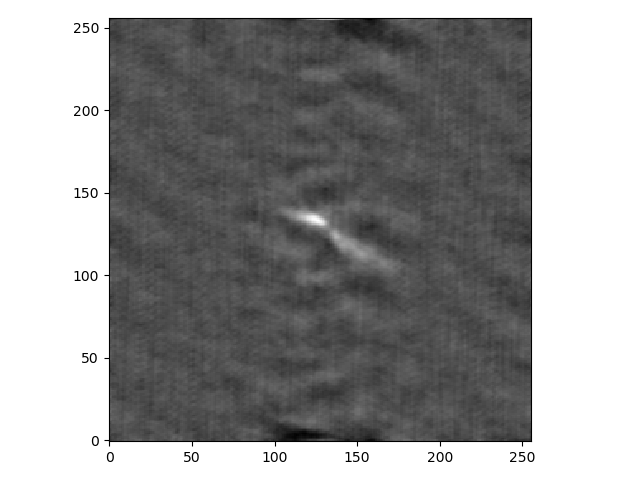
\includegraphics[height=0.275\textheight]{intensity.png}
\vspace{-1em}
\caption{The integrated intensity map of the outflow. Here the units of the axes are pixels in the FITS file and the values themselves are brightness temperature (\si{\kelvin}). The bottom right lobe is blueshifted and the top left is redshifted.}
\end{figure}

\newpage
\item We generate the Hubble diagram using the \texttt{pvextractor} package in Python. Here the path was chosen to be the end of the redshifted lobe, through the central point between the lobes, and the end of the blue blueshifted lobe. Looking at the $p{-}v$ diagram (Figure 3), we notice that there seems to be somewhat of a bimodal distribution in the velocity corresponding to pixels $24$ and $36$. From the FITS file pixel $36$ in the velocity roughly corresponds to $v = 0$, so we can assume this to be noise from the interferometer. If we take pixel $24$ as the true signal, then we have that the velocity peaks at around $3.7$ \si{\kilo\meter/\second}. Dividing the combined length of the outflows (${\sim}0.729$ \si{pc}) by this velocity, we obtain a dynamical age of roughly $0.192$ \si{Myr}. This seems to be a good measure of the source's actual age, as it falls within the age range of a class 0 protostar. This Hubble diagram suggests that accretion is relatively constant, as this velocity peak is roughly uniform throughout the outflow. However we also note that at farther distances there is a blend of higher velocities, which suggests that overall the accretion is slowing down. This agrees with our expectations, as accretion rate should be the highest during the class 0 stage and go down as the envelope gets consumed or blown away by the forming star.

\begin{figure}[h]
\centering
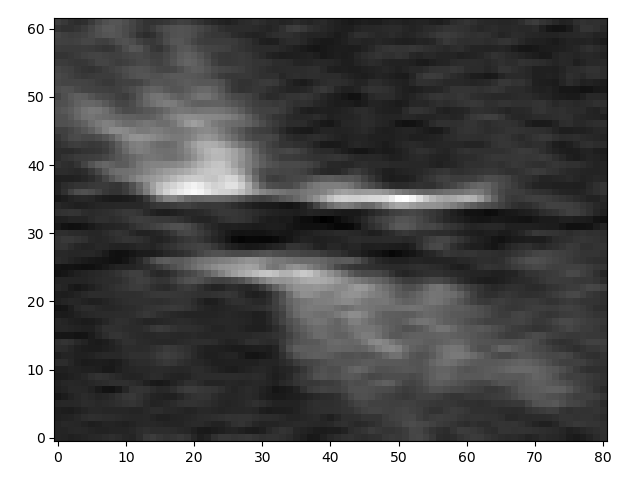
\includegraphics[height=0.275\textheight]{hubble.png}
\vspace{-1em}
\caption{The Hubble diagram ($p{-}v$) of the outflow. Again the axes here represent pixels; the $x$-axis represents the pixel distance and the $y$-axis represent the FITS file's velocity in terms of pixels.}
\end{figure}

\item Using our old code from Homework 2, we obtain an outflow mass of $0.0669$ \si{\msun} for the outflow. Assuming that this outflow is actually about $0.2$ \si{Myr} old, we can assume a mass ejection rate (from outflows) of $3.475\cdot10^{-7}$ \si{\msun/yr}. The outflow mass rate is related to the accretion rate by the equation $\dot{m}_{0} \approx f_{0}\dot{m}_{*}$, where $f_{0} \approx 0.1{-}0.3$. This gives us an estimated accretion rate of $(1.158{-}3.475)\cdot10^{-6}$ \si{\msun/yr}, which is reasonable. Finally, from Offner \& Arce (2014) we see that after about $0.2$ \si{Myr}, a star's mass is roughly four times greater than the mass launched in outflows (although this simulation admittedly had much higher collimation). If only a third of the calculated outflow mass is actually launched, this gives an estimate of roughly $0.0891$ \si{\msun}, which although on the low side is not entirely out of the realm of possibility for a class 0 protostar. 
\end{tight_enumerate}



\end{document}